\documentclass[]{article}
\usepackage{multicol}
\usepackage{setspace}
\usepackage{mathrsfs}
\usepackage{graphicx}
\usepackage{subcaption}
\usepackage[labelfont=bf]{caption}
\usepackage{amsmath}

\setcounter{tocdepth}{2} 

%opening
\title{Analog and Digital Communications - Formulae and Identities}
\begin{document}
\maketitle

\tableofcontents
\newpage

\section{Signals and Systems}
%\begin{multicols}{2}
	
\subsection{Basics}
\subsubsection{Normalized Energy}
The normalized energy content $E$ of a signal $x(t)$ is defined as

\begin{equation} E = \int_{-\infty}^{\infty} |x(t)|^{2}dt \label{norm_energy} \end{equation}

\subsubsection{Average Power}
The normalized average power $P$ of a signal $x(t)$ is defined as

\begin{equation} P = \lim_{T \to \infty} \frac{1}{T} \int_{-T/2}^{T/2} |x(t)|^{2} dt\label{norm_power}\end{equation} 

\subsubsection{Dirac Delta Function}
The unit impulse function (or Dirac delta function) $\delta (t)$ is defined as

\begin{equation}\delta (t) = \int_{-\infty}^{\infty} \phi(t) \delta (t)dt = \phi(0)\label{dirac_def}\end{equation}
where $\phi (t) $ is any test function continuous at $t=0$. The unit impulse function is a \textit{generalized function}.

\subsubsection{Derivatives of Generalized Functions}
The derivative $g'(t)$ of a generalized function $g(t)$ is defined by
\begin{equation}\int_{-\infty}^{\infty} g'(t) \phi(t) dt = - \int_{-\infty}^{\infty} g(t) \phi '(t)dt\label{gen_func_def} \end{equation}

\subsubsection{Complex Fourier Series}
The Fourier series for a signal $x(t)$ is defined as

\begin{equation} x(t) = \sum_{n=-\infty}^{\infty} c_{n} e^{jn\omega_{0}\label{complex_fourier_series} t}\end{equation}
where $\omega_{0}$ is the fundamental angular frequency.
The Fourier coefficients $c_{n}$ are given by

\begin{equation} c_{n} = \frac{1}{T_{0}} \int_{-T_{0}/2}^{T_{0}/2} x(t) e^{-jn\omega_{0}t} dt\label{complex_fourier_coefs} \end{equation}
A plot of $|c_{n}|$ vs $\omega$ is called the amplitude spectrum. A plot of $\theta_{n}$ (the phase constants of $c_{n}$) vs $\omega$ is called the phase spectrum. Together these are referred to as the frequency spectra.
\subsubsection{Parseval's Theorem}
Parseval's theorem states that for a periodic signal $x(t)$
\begin{equation} \frac{1}{T_{0}} \int_{-T_{0}/2}^{T_{0}/2} |x(t)|^2dt = \sum_{n=-\infty}^{\infty} |c_{n}|^2\label{parsevals_theorem} \end{equation}

\subsubsection{Fourier Transform}
The Fourier transform, $\mathscr{F}$, of a signal $x(t)$ is given by
\begin{equation} X(\omega) = \mathscr{F}[x(t)] = \int_{-\infty}^{\infty}x(t)e^{-j\omega t}dt\label{complex_fourier_transform} \end{equation}

\subsubsection{Inverse Fourier Transform}
The inverse Fourier transform of $X(\omega)$,  $\mathscr{F}^{-1}$, is given by
\begin{equation} x(t) = \frac{1}{2\pi} \int_{-\infty}^{\infty}X(\omega)e^{j\omega t} d\omega\label{inv_complex_fourier_transform} \end{equation}

\subsection{Properties of the Fourier Transform}
$ x(t) \longleftrightarrow X(\omega)$ denotes a Fourier transform pair.
\subsubsection{Linearity}
\begin{equation} a_{1} x_{1}(t) + a_{2} x_{2}(t) \longleftrightarrow a_{1} X_{1}(\omega) + a_{2} X_{2}(\omega)\label{fourier_linearity} \end{equation}
\subsubsection{Time Shifting}
\begin{equation} x(t-t_{0}) \longleftrightarrow X(\omega)e^{-j\omega t_{0}}\label{fourier_time_shifting} \end{equation}
\subsubsection{Frequency Shifting}
\begin{equation} x(t)e^{j\omega_{0} t} \longleftrightarrow X(\omega - \omega_{0})\label{fourier_frequency_shifting} \end{equation}
\subsubsection{Scaling}
\begin{equation} x(at) \longleftrightarrow \frac{1}{|a|}X(\frac{\omega}{a})\label{fourier_scaling} \end{equation}
\subsubsection{Time Reversal}
\begin{equation} x(-t) \longleftrightarrow X(-\omega)\label{fourier_time_reversal} \end{equation}
\subsubsection{Duality}
\begin{equation} X(t) \longleftrightarrow 2\pi x(-\omega)\label{fourier_duality} \end{equation}
\subsubsection{Differentiation}
Time differentiation
\begin{equation} x'(t) = \frac{d}{dt}x(t) \longleftrightarrow j\omega X(\omega)\label{fourier_time_differentiation}\end{equation}
Frequency differentiation
\begin{equation} (-jt)x(t) \longleftrightarrow X'(\omega) = \frac{d}{d\omega}X(\omega)\label{fourier_freq_differentiation} \end{equation}
\subsubsection{Integration}
\begin{equation} \int_{-\infty}^{t} x(\tau)d\tau \longleftrightarrow \frac{1}{j\omega}X(\omega) + \pi X(0)\delta(\omega)\label{fourier_integration}\end{equation}

\subsubsection{Modulation Theorem}
\begin{equation} x(t)cos(\omega_{0}t) \longleftrightarrow \frac{1}{2}X(\omega - \omega_{0}) + \frac{1}{2}X(\omega + \omega_{0})\label{modulation_theorem}\end{equation}

\subsection{Convolutions and Correlation}
The convolution of two signals $x_{1}(t)$ and $x_{2}(t)$ is
\begin{equation} x_{1}(t) * x_{2}(t) = \int_{-\infty}^{\infty} x_{1}(\tau) x_{2}(t-\tau)d\tau\label{convolution_def} \end{equation}
\subsubsection{Time Convolution Theorem}
\begin{equation} x_{1}(t) * x_{2}(t) \longleftrightarrow X_{1}(\omega) X_{2}(\omega)\label{time_convolution_thrm}\end{equation} 
\subsubsection{Frequency Convolution Theorem}
\begin{equation}x_{1}(t)x_{2}(t) \longleftrightarrow \frac{1}{2\pi}X_{1}(\omega)*X_{2}(\omega)\label{freq_convolution_thrm} \end{equation}
\subsubsection{Cross-Correlation}
The cross correlation $R_{12}(\tau)$ of signals $x_{1}(t)$ and $x_{2}(t)$ is defined by
\begin{equation}R_{12}(\tau) = \int_{-\infty}^{\infty}x_{1}(t)x_{2}(t-\tau)dt\label{cross_corr_defn} \end{equation}
\subsubsection{Autocorrelation}
The autocorrelation is defined as the cross-correlation of a signal $x_{1}(t)$ with itself, $R_{11}(\tau)$.
\subsubsection{Energy Spectral Density}
The energy spectral density $S_{11}$ of a signal $x_{1}(t)$ is given by
\begin{equation}S_{11}(\omega) = \mathscr{F}[R_{11}(\tau)] = \int_{-\infty}^{\infty}R_{11}(\tau)e^{-j\omega \tau}d\omega\label{energy_spectral_density} \end{equation}
\subsection{Linear Time-Invariant Systems}
Linear time-invariant (linear time-invariant) systems have several properties, as follows. Suppose $\mathcal{F}$ is an operator representing the action of a system with output $y(t)$.
\subsubsection{Additivity}
\begin{equation}\mathcal{F}[x_{1}(t) +x_{2}(t)] = \mathcal{F}[x_{1}(t)] + \mathcal{F}[x_{2}(t)]\label{lti_additivity}\end{equation}
\subsubsection{Homogeneity}
\begin{equation}\mathcal{F}[ax(t)] = a\mathcal{F}[x(t)]\label{lti_homogeneity} \end{equation}
\subsubsection{Time-Invariance}
\begin{equation}\mathcal{F}[x(t-t_{0})] = y(t-t_{0})\label{lti_time_invariance} \end{equation}
\subsubsection{Impulse Response}
The impulse response $h(t)$ of an LTI system is the response of the system with a delta function input
\begin{equation} h(t) = \mathcal{F}[\delta(t)] \label{impulse_response_def}\end{equation}
\subsubsection{Response to Arbitrary Inputs}
The response of an LTI system to an arbitrary input can be expressed in terms of a convolution with the impulse response of the system
\begin{equation}y(t) = x(t)*h(t)=\int_{-\infty}^{\infty}x(\tau)h(t-\tau)d\tau\label{lti_system_response} \end{equation}
\subsubsection{Causality}
A signal $x(t)$ is causal if, for $t<0$, $x(t)=0$.
\subsubsection{Frequency Response}
Using the time convolution theorem ($\ref{time_convolution_thrm}$) on the response of an LTI system ($\ref{lti_system_response}$), we find that
\begin{equation} Y(\omega) = X(\omega)H(\omega) \label{freq_response} \end{equation}
where $Y(\omega)=\mathscr{F}[y(t)]$ and $H(\omega)=\mathscr{F}[h(t)]$. We refer to $H(\omega)$ as the \textit{frequency response} or \textit{transfer function}.
\subsubsection{Input and Output Spectral Densities}
\begin{equation} S_{yy}(\omega) = |H(\omega)|^{2} S_{xx}(\omega)  \end{equation}
\begin{equation}\bar{S}_{yy}(\omega) = |H(\omega)|^{2} \bar{S}_{xx}(\omega)  \end{equation}

%\end{multicols}
\newpage
\section{Amplitude Modulation}
Modulation is defined as the process by which some characteristic of a carrier signal is varied in accordance with a modulating signal (message signal). There are two basic types of analog modulation; continuous wave (CW) modulation and pulse modulation.

%\begin{multicols}{2}
\subsection{Continuous-Wave Modulation}
In continuous-wave modulation, a sinusoidal signal is used as a carrier signal. The modulated carrier signal $x_{c}(t)$ is given by
\begin{equation} x_{c}(t) = A(t)cos[\omega_{c}t + \phi (t)] \label{cw_carrier_signal} \end{equation}
Let $m(t)$ be the message signal.
\subsubsection{Double-Sideband Modulation}
Double-sideband (DSB) modulation occurs when $m(t) = A(t)$. The DSB modulated signal $x_{DSB}(t)$ is then given by
\begin{equation} x_{DSB}(t) = m(t)cos(\omega_{c}t) \label{dsb_carrier_signal} \end{equation}
By applying the modulation theorem ($\ref{modulation_theorem}$), we obtain the following
\begin{equation} X_{DSB}(\omega) = \frac{1}{2}M(\omega - \omega_{c}) + \frac{1}{2}M(\omega + \omega_{c}) \label{dsb_fourier_transform} \end{equation}
See figure $\ref{fig:dsb_modulation}$ for an example.

\begin{figure}[h!]
	\centering
	\begin{subfigure}[b]{0.3\textwidth}
		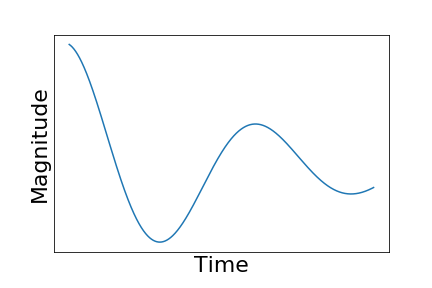
\includegraphics[width=\textwidth]{figs/amplitude_modulation/dsb/message_signal.png}
		\caption{Message signal}
		\label{fig:dsb_message_signal}
	\end{subfigure}
	~ %add desired spacing between images, e. g. ~, \quad, \qquad, \hfill etc. 
	%(or a blank line to force the subfigure onto a new line)
	\begin{subfigure}[b]{0.3\textwidth}
		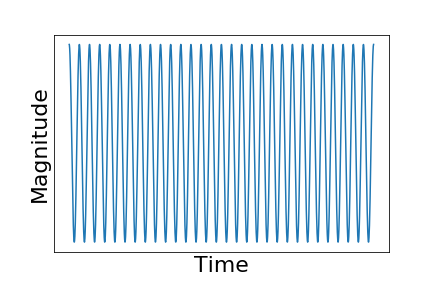
\includegraphics[width=\textwidth]{figs/amplitude_modulation/dsb/carrier_signal.png}
		\caption{Carrier signal}
		\label{fig:dsb_carrier_signal}
	\end{subfigure}
	~ %add desired spacing between images, e. g. ~, \quad, \qquad, \hfill etc. 
	%(or a blank line to force the subfigure onto a new line)
	\begin{subfigure}[b]{0.3\textwidth}
		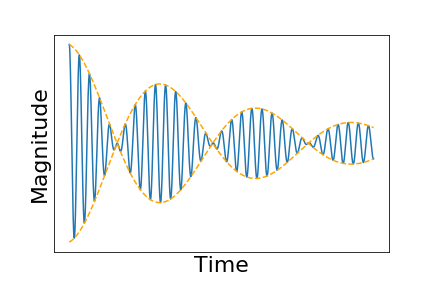
\includegraphics[width=\textwidth]{figs/amplitude_modulation/dsb/modulated_signal.png}
		\caption{Modulated signal}
		\label{fig:dsb_modulated_signal}
	\end{subfigure}
	\begin{subfigure}[b]{0.3\textwidth}
		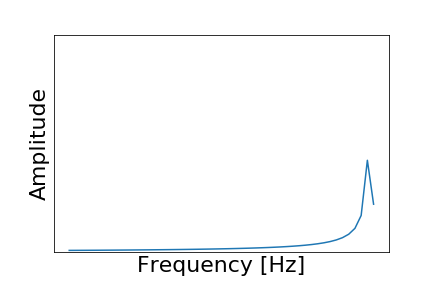
\includegraphics[width=\textwidth]{figs/amplitude_modulation/dsb/message_signal_freq.png}
		\caption{Message signal}
		\label{fig:dsb_message_signal_freq}
	\end{subfigure}
	~ %add desired spacing between images, e. g. ~, \quad, \qquad, \hfill etc. 
	%(or a blank line to force the subfigure onto a new line)
	\begin{subfigure}[b]{0.3\textwidth}
		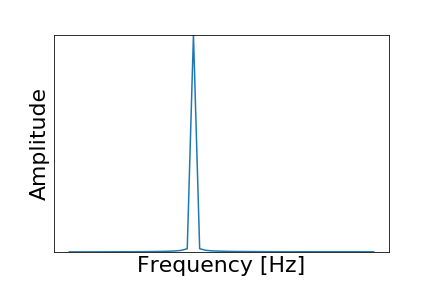
\includegraphics[width=\textwidth]{figs/amplitude_modulation/dsb/carrier_signal_freq.png}
		\caption{Carrier signal}
		\label{fig:dsb_carrier_signal_freq}
	\end{subfigure}
	~ %add desired spacing between images, e. g. ~, \quad, \qquad, \hfill etc. 
	%(or a blank line to force the subfigure onto a new line)
	\begin{subfigure}[b]{0.3\textwidth}
		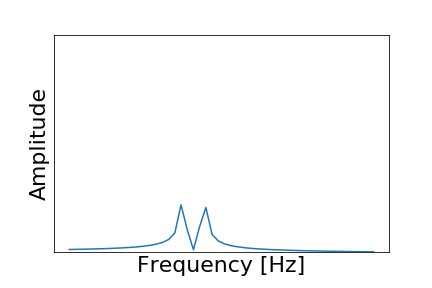
\includegraphics[width=\textwidth]{figs/amplitude_modulation/dsb/modulated_signal_freq.png}
		\caption{Modulated signal}
		\label{fig:dsb_modulated_signal_freq}
	\end{subfigure}
	\caption{Modulating a message signal onto a carrier signal with DSB modulation. Plots (a), (b) and (c) display signals in the time domain, whereas (d), (e) and (c) display the signals in the frequency domain. Note how the carrier signal frequency gets split into two smaller peaks. These are referred to as the upper and lower sidebands.}\label{fig:dsb_modulation}
\end{figure}

\subsubsection{Ordinary Amplitude Modulation}
Ordinary amplitude modulation (AM) varies the carrier signal amplitude linearly with respect to the message signal as follows

\begin{equation} x_{c}(t) = [1 + k_{a}m(t)]A(t)cos(\omega_{c}t) \end{equation}
where $|k_{a}m(t)|<1$.

\begin{figure}[h!]
	\centering
	\begin{subfigure}[b]{0.3\textwidth}
		\includegraphics[width=\textwidth]{figs/amplitude_modulation/am/message_signal.png}
		\caption{Message signal}
		\label{fig:am_message_signal}
	\end{subfigure}
	~ %add desired spacing between images, e. g. ~, \quad, \qquad, \hfill etc. 
	%(or a blank line to force the subfigure onto a new line)
	\begin{subfigure}[b]{0.3\textwidth}
		\includegraphics[width=\textwidth]{figs/amplitude_modulation/am/carrier_signal.png}
		\caption{Carrier signal}
		\label{fig:am_carrier_signal}
	\end{subfigure}
	~ %add desired spacing between images, e. g. ~, \quad, \qquad, \hfill etc. 
	%(or a blank line to force the subfigure onto a new line)
	\begin{subfigure}[b]{0.3\textwidth}
		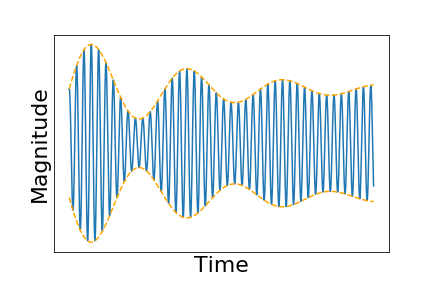
\includegraphics[width=\textwidth]{figs/amplitude_modulation/am/modulated_signal.png}
		\caption{Modulated signal}
		\label{fig:am_modulated_signal}
	\end{subfigure}
	\begin{subfigure}[b]{0.3\textwidth}
		\includegraphics[width=\textwidth]{figs/amplitude_modulation/am/message_signal_freq.png}
		\caption{Message signal}
		\label{fig:am_message_signal_freq}
	\end{subfigure}
	~ %add desired spacing between images, e. g. ~, \quad, \qquad, \hfill etc. 
	%(or a blank line to force the subfigure onto a new line)
	\begin{subfigure}[b]{0.3\textwidth}
		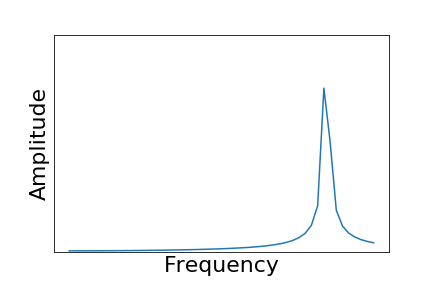
\includegraphics[width=\textwidth]{figs/amplitude_modulation/am/carrier_signal_freq.png}
		\caption{Carrier signal}
		\label{fig:am_carrier_signal_freq}
	\end{subfigure}
	~ %add desired spacing between images, e. g. ~, \quad, \qquad, \hfill etc. 
	%(or a blank line to force the subfigure onto a new line)
	\begin{subfigure}[b]{0.3\textwidth}
		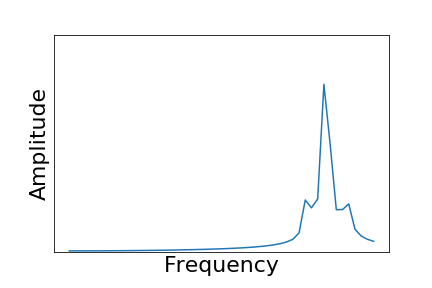
\includegraphics[width=\textwidth]{figs/amplitude_modulation/am/modulated_signal_freq.png}
		\caption{Modulated signal}
		\label{fig:am_modulated_signal_freq}
	\end{subfigure}
	\caption{Modulating a message signal onto a carrier signal with AM modulation. Plots (a), (b) and (c) display signals in the time domain, whereas (d), (e) and (c) display the signals in the frequency domain.}\label{fig:am_modulation}
\end{figure}

\subsubsection{Single-Sideband Modulation}
There are two types of single single sideband (SSB) modulation; upper sideband and lower sideband. They can both be generated by phase-shifting the message signal by $\frac{\pi}{2}$, resulting in a modulated signal given as below
\begin{equation} x_{SSB}(t) = m(t)cos(\omega_{c}t) \mp \hat{m}(t)sin(\omega_{c}t) \end{equation}
where the difference results in an upper sideband and the sum results in the lower sideband.
\begin{figure}[h!]
	\centering
	\begin{subfigure}[b]{0.3\textwidth}
		\includegraphics[width=\textwidth]{figs/amplitude_modulation/ssb/message_signal.png}
		\caption{Message signal}
		\label{fig:ssb_message_signal}
	\end{subfigure}
	~ %add desired spacing between images, e. g. ~, \quad, \qquad, \hfill etc. 
	%(or a blank line to force the subfigure onto a new line)
	\begin{subfigure}[b]{0.3\textwidth}
		\includegraphics[width=\textwidth]{figs/amplitude_modulation/ssb/carrier_signal.png}
		\caption{Carrier signal}
		\label{fig:ssb_carrier_signal}
	\end{subfigure}
	~ %add desired spacing between images, e. g. ~, \quad, \qquad, \hfill etc. 
	%(or a blank line to force the subfigure onto a new line)
	\begin{subfigure}[b]{0.3\textwidth}
		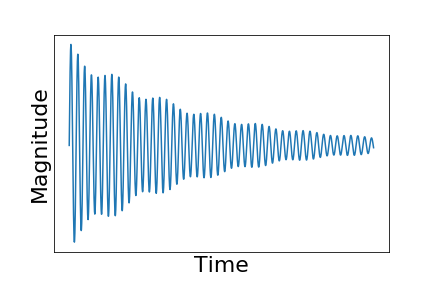
\includegraphics[width=\textwidth]{figs/amplitude_modulation/ssb/modulated_signal.png}
		\caption{Modulated signal}
		\label{fig:ssb_modulated_signal}
	\end{subfigure}
	\begin{subfigure}[b]{0.3\textwidth}
		\includegraphics[width=\textwidth]{figs/amplitude_modulation/ssb/message_signal_freq.png}
		\caption{Message signal}
		\label{fig:ssb_message_signal_freq}
	\end{subfigure}
	~ %add desired spacing between images, e. g. ~, \quad, \qquad, \hfill etc. 
	%(or a blank line to force the subfigure onto a new line)
	\begin{subfigure}[b]{0.3\textwidth}
		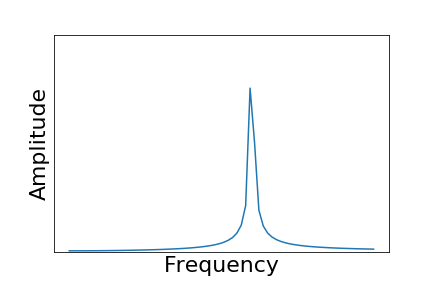
\includegraphics[width=\textwidth]{figs/amplitude_modulation/ssb/carrier_signal_freq.png}
		\caption{Carrier signal}
		\label{fig:ssb_carrier_signal_freq}
	\end{subfigure}
	~ %add desired spacing between images, e. g. ~, \quad, \qquad, \hfill etc. 
	%(or a blank line to force the subfigure onto a new line)
	\begin{subfigure}[b]{0.3\textwidth}
		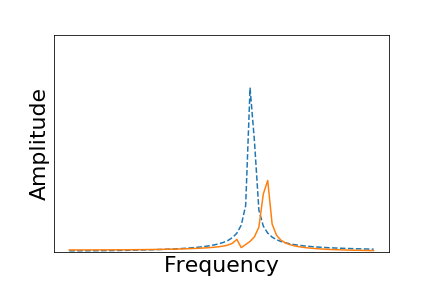
\includegraphics[width=\textwidth]{figs/amplitude_modulation/ssb/modulated_signal_freq.png}
		\caption{Modulated signal}
		\label{fig:ssb_modulated_signal_freq}
	\end{subfigure}
	\caption{Modulating a message signal onto a carrier signal with upper SSB modulation. Plots (a), (b) and (c) display signals in the time domain, whereas (d), (e) and (c) display the signals in the frequency domain.}\label{fig:ssb_modulation}
\end{figure}
\subsubsection{Vestigial-Sideband Modulation}
Vestigial-sideband modulation is similar to DSB, except one sideband is attenuated. This is a compromise between DSB and SSB. Vestigial-sideband modulation is performed on top of DSB modulation, with a vestigial-sideband filter applied as the final step.
\subsection{Frequency Translation and Mixing}
Test

\newpage
\section{Angle Modulation}
Angle modulation includes both phase modulation (PM) and frequency modulation (FM). We again use a sinusoidal carrier signal 
\begin{equation}x_{c}(t) = Acos[\omega_{c}t+\phi(t)] \label{message_signal_sinusoidal_mod}\end{equation}
However, instead of modifying the amplitude $A$, we modify the phase angle $\phi(t)$ by making it a function of the message signal $m(t)$.


Let $\theta(t) = \omega_{c}t+\phi(t)$. Then the instantaneous radian frequency of $x_{c}(t)$ is given by 
\begin{equation} \omega_{inst} = \frac{d \theta(t)}{dt} = \omega_{c}+ \frac{d \phi(t)}{dt} \end{equation} 
\subsection{Phase Modulation}
In phase modulation, we let the phase angle $\phi(t) = k_{p}m(t)$, where $k_{p}$ is the phase deviation constant.
\subsection{Frequency Modulation}
In frequency modulation, we set $\frac{d\phi(t)}{dt} = k_{f}m(t)$, where $k_{f}$ is the frequency deviation constant. Integrating over $m(t)$, we find the following expression for $\phi(t)$
\begin{equation} \phi(t) = k_{f} \int_{t_{0}}^{t} m(\lambda) + \phi(t_{0}) \end{equation}
We usually let $t_{0} = -\infty$ and $\phi(-\infty)=0$.
\subsection{Sinusoidal Angle Modulation}
Sinusoidal message signals result in a phase angle of
\begin{equation} \phi(t) = \beta sin(\omega_{m}t) \label{sinusoidal_mod_phase_angle}\end{equation}
$\beta$ is referred to as the modulation index and gives the maximum value of phase deviation. $\beta$ can be expressed as 
\begin{equation} \beta = \frac{\Delta \omega}{\omega_{m}} \end{equation}
where $\Delta \omega$ is the maximum frequency deviation. Substituting ($\ref{sinusoidal_mod_phase_angle}$) into ($\ref{message_signal_sinusoidal_mod}$) and expressing it as a Fourier series, we obtain
\begin{equation} x_{c}(t) = A \sum_{n=-\infty}^{\infty} J_{n}(\beta)cos(\omega_{c}+n\omega_{m})t \end{equation}
where $J_{n}(\beta)$ are Bessel functions of order $n$. Three things should be noted:
\begin{enumerate}
	\item The signal is composed of a carrier frequency with infinite harmonic sidebands.
	\item The aplitude is dependant on $J_{n}(\beta)$, which gets smaller with larger values of $|n|$.
	\item $\beta$ also determines the number of significant spectral lines, with smaller $\beta$ resulting in fewer significant sidebands and greater $\beta$ resulting in more numerous significant sidebands.
\end{enumerate}
\subsection{Bandwidth of Angle Modulated Signals}
\subsubsection{Sinusoidal Modulation}
The bandwidth $W_{B}$ of a signal with sinusoidal modulation is approximately given as follows
\begin{equation} W_{B} \approx 2(\beta + 1)\omega_{m} \end{equation}
\subsubsection{Arbitrary Modulation}
The Deviation radio $D$ is defined as
\begin{equation} D = \frac{\Delta \omega}{\omega_{M}} \end{equation}
for a message signal bandwidth $\omega_{M}$. The bandwidth of the modulated signal is then given as
\begin{equation} W_{B} \approx 2(D +1)\omega_{M} \end{equation}
$W_{B}$ contains $98\%$ of signal power.
\section{Digital Transmission of Analog Signals}
\subsection{Pulse Code Modulation}
Pulse code modulation (PCM) consists of three main steps: sampling, quantisation and encoding. The sampled signal must be \textit{bandwidth limited} - ie it must be composed of a finite number of frequencies.
\subsubsection{Pulse Amplitude Modulation}
Pulse amplitude modulation (PAM) utilises a periodic train of rectangular pulses as the carrier signal $x_{c}(t)$. The modulated signal $x_{PAM}(t)$ is then given by the discrete convolution of the message signal $m(t)$ and the carrier signal
\begin{equation} x_{PAM}(t) = m(t)*x_{c}(t) = \sum_{n=-\infty}^{\infty} m(nT_{s})x_{c}(t-nT_{s}) \end{equation}
where $T_{s}$ is the sampling frequency.
\subsubsection{Quantising Error}
Once the signal has been modulated, thereby quantising in time, its amplitude must also be quantised. There is an error associated with uniform quantisation that is referred to as quantising error or quantising noise. Given an amplitude step size of $\Delta_{A}$, the quantising error $q_{e}$ varies uniformly over $[-\frac{\Delta_{A}}{2}, \frac{\Delta_{A}}{2}]$. The expected value of $q_{e}^{2}$ is thus
\begin{equation} \langle q_{e}^{2} \rangle = \frac{1}{\Delta_{A}} \int_{-\Delta_{A}/2}^{\Delta_{A}/2} q_{e}^{2}dq_{e} = \frac{\Delta_{A}^{2}}{12} \end{equation}
\subsubsection{Non-uniform Quantisation}
Oftentimes signals are not evenly distributed over their range of values. In these situations, it is better to use non-uniform quantisation that allows for finer discretisation in ranges of amplitudes where signal values are more likely to be. A typical method of non-uniform quantisation is to first use a non-linear \textit{compression} of the original signal followed by a uniform quantisation of the compressed signal. A common compression used is the \textit{$\mu$ law}
\begin{equation} y = \frac{ln(1+\mu|m/m_{p}|)}{ln(1+\mu)}sgn(m), \qquad \bigg|\frac{m}{m_{p}}\bigg| \leq 1 \end{equation}
where $\mu$ is a positive constant, $m_{p}$ is the maximum signal amplitude and $sgn(m) = 1$ if $m>0$ and $-1$ otherwise.

Another common compression is the \textit{A law}, given by
\begin{equation} y=\begin{cases}
\frac{A}{1+ln(A)}( \frac{m}{m_{p}}), & |\frac{m}{m_{p}}|\leq \frac{1}{A}\\
\frac{(1+ln(A)|m/m_{p}|)}{1+ln(A)}sgn(m), & \frac{1}{A}\leq |\frac{m}{m_{p}}|\leq 1.
\end{cases} \end{equation}
\subsubsection{Bandwidth Requirements}
test




\bibliographystyle{amsplain}

\bibliography{refs}
%\end{multicols}
\end{document}
